\documentclass[a4paper]{article}

\usepackage{graphicx}
\usepackage{amsmath,amssymb}
\usepackage{minted}
\usepackage{multirow}
\usepackage{float}
\usepackage{algorithm}
\usepackage{algpseudocode}
\usepackage{todonotes}
\usepackage{forest}
\usepackage{xstring}
\usepackage{xcolor}
\usepackage[most]{tcolorbox}
\usepackage{xparse}
\usepackage{natbib}
\usepackage{adjustbox}

\usetikzlibrary{graphs,graphdrawing}
\usegdlibrary{layered}

% for external graphviz
\input{/home/donkarlo/Dropbox/repo/nd_language_ai_project/src/nd_language_ai/formal/computer/programming/tex/latex/code_clips/external_graphviz.tex}

% for tags
\input{/home/donkarlo/Dropbox/repo/nd_language_ai_project/src/nd_language_ai/formal/computer/programming/tex/latex/part/control_sequence/kind/semtag/semtag.tex}

% for links
\input{/home/donkarlo/Dropbox/repo/nd_language_ai_project/src/nd_language_ai/formal/computer/programming/tex/latex/code_clips/seehere.tex}

% for nested lists and sections
\input{/home/donkarlo/Dropbox/repo/nd_language_ai_project/src/nd_language_ai/formal/computer/programming/tex/latex/code_clips/deep_structure.tex}

\title{}
\date{}
\author{Mohammad Rahmani}

\begin{document}
   \maketitle

   Max ist in den Ferien bei den Großeltern zu Besuch, die ein kleines Restaurant besitzen. Das ist toll, denn Max kann jeden Tag im Restaurant essen und von der Speisekarte wählen, was ihm gefällt. Heute hat er sich für Hühnchen mit Kartoffeln entschieden. Als Getränk hat er Limonade bestellt. Und als Dessert gibt es eine große Portion Eis.

   Mittags ist im Restaurant seiner Großeltern noch nicht viel los. Es gibt nur wenige Gäste. Außer Max befindet sich nur ein weiterer Gast im Restaurant - eine ältere Dame. Sie hat eben die Rechnung bestellt und trinkt noch ihren Kaffee. Max‘ Großvater, der Kellner ist, hat die Rechnung schon an der Kasse ausgedruckt und auf das Tablett gelegt, auf dem auch ein Eis als Dessert für Max steht.

   Plötzlich hört man aus der Küche ein lautes Geschrei. Erst rennt eine Katze durch das Restaurant, dann der Koch. Oh nein! Die Katze hat sich in der Küche einen Fisch gestohlen und flitzt damit(ba an, mit dem Fisch) zur Tür. Der Koch, der den Fisch gerade noch zubereiten wollte, rennt wütend hinterher.

   „Gut, dass die Katze heute Appetit auf Fisch hatte und nicht auf Hühnchen,“ denkt sich Max, nimmt Messer und Gabel und beginnt zu essen.
   
   \begin{figure}[H]
      \centering
      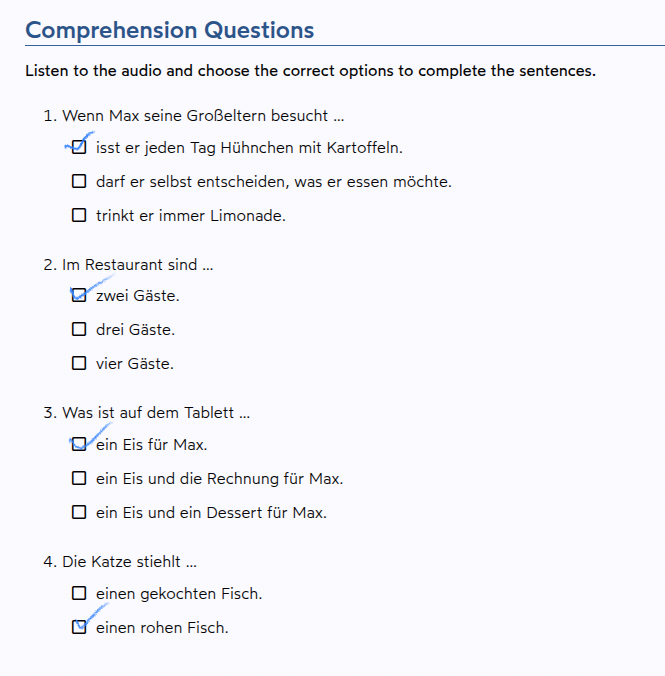
\includegraphics[width=0.9\textwidth]{img_0.png}
   \end{figure}   
   \bibliographystyle{plainnat}
   \bibliography{/home/donkarlo/Dropbox/repo/nd_shared_research/bibliography/bibliography.bib}
\end{document}
